\chapter{ARSITEKTUR SISTEM}

Jika membahas arsitektur sistem, maka akan ada beberapa diagram yang terbentuk untuk memudahkan dalam penjelasan sebuah sistem. Penggambaran diagram arsitektur sistem ini berkembang mengikuti model pemrogramannya, dimana dahulu ada yang dikenal dengan \textit{flow-chart} yang menggambarkan alur proses sebuah sistem aplikasi berjalan, mulai dari awal, sampai sistem aplikasi tersebut ditutup dan selesai digunakan, karena memang model pemrograman pada saat ini berbentuk prosedural. 

Namun berkembangnya jaman, dikenal istilah pemrograman berorientasi objek, yang salah satu bahasa pemrogramannya adalah Java. Dengan menggunakan Java, maka diagram \textit{flow-chart} tidak akan bisa melakukan penggambaran alurnya karena pola pada pemrograman berorientasi objek selalu melompat dari satu kelas ke kelas yang lain, dari satu \textit{method} ke \textit{method} yang lain. Maka dibutuhkan penggambaran desain arsitektur yang lain selain \textit{flow-chart}, salah satunya adalah \textit{Unified Modelling Language} (UML).

UML sendiri sebetulnya hanya menggambarkan 2 (dua) sudut pandang dalam pemodelan sistem, yaitu :

\begin{itemize}
  \item \textit{Static view}, yang menekankan pada struktur sistem yang bersifat statis seperti objek, operasi, dan relasi.
  
  \item \textit{Dynamic view}, yang menekankan pada sifat atau tingkah laku dari sistem yang menunjukkan interaksi antar objek didalamnya.
\end{itemize}

\section{Diagram \textit{Use-Case}}

Hal yang pertama digambarkan adalah skenario penggunaan aplikasi secara umum, akan berangkat dari diagram \textit{use-case} seperti pada gambar \ref{fig:uml-use-case} :

\begin{figure}[H]
  \centering
  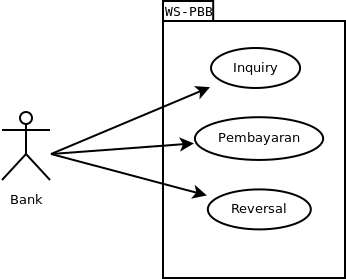
\includegraphics[width=0.5\textwidth]{./resources/uml/uml-use-case}
  \caption{Diagram \textit{use-case}}
  \label{fig:uml-use-case}
\end{figure}

Dari diagram \textit{use-case} diatas, skenarionya adalah bahwa Bank sebagai tempat pembayaran dapat melakukan \textit{request} pada ketiga hal yang disediakan oleh \textit{web services} PBB di DPPK. yaitu :

\begin{itemize}
  \item \textit{Inquiry}
  \item Pembayaran
  \item Reversal
\end{itemize}

Untuk melihat masing-masing proses pada skenario diatas, ada pada diagram \textit{activity} yang dibahas pada bagian selanjutnya. 

\section{Diagram \textit{Activity}}

Diagram \textit{activity} ini akan menunjukan aktivitas yang terjadi untuk setiap skenario pada diagram \textit{use-case}. Berikut skema diagram dari masing-masing skenario yang terbagi menjadi 3 (tiga) diagram berdasarkan jumlah skenario pada diagram \textit{use-case} :

\subsection{Diagram \textit{Activity} Untuk \textit{Inquiry}}

Bagan diagram \textit{activity} untuk \textit{inquiry} ini seperti ditunjukan pada gambar \ref{fig:act-inquiry} :

\begin{figure}[H]
  \centering
  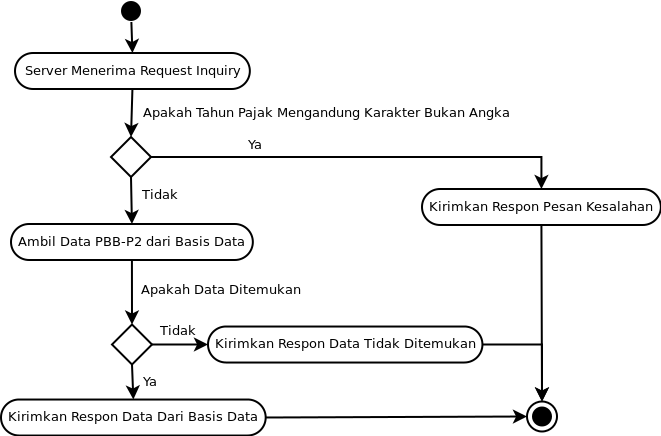
\includegraphics[width=0.8\textwidth]{./resources/uml/uml-act-inquiry}
  \caption{Diagram \textit{Activity} untuk \textit{Inquiry}}
  \label{fig:act-inquiry}
\end{figure}

Aktivitas akan dimulai dari lingkaran penuh di atas, yang kemudian didahului oleh \textit{client} yang melakukan \textit{request} untuk \textit{inquiry} data PBB-P2, hal yang pertama dilakukan adalah melakukan pemeriksaan informasi tahun pajak yang diminta, apakah mengandung karakter atau tidak.

Bila Tahun pajak terisi dengan angka yang wajar, maka aplikasi \textit{web services} akan melakukan koneksi dengan basis data SISMIOP untuk mengambil informasi-informasi yang dibutuhkan oleh \textit{client}.

Bila data tidak ditemukan dalam basis data, maka aplikasi \textit{web services} akan mengirimkan informasi kepada \textit{client} bahwa data yang diminta tidak ditemukan, namun bila data ditemukan, maka disusun dalam format JSON dan dikirimkan ke \textit{client} sebagai respon atas \textit{request} tersebut.

Sampai sini aktivitas selesai.

\subsection{Diagram \textit{Activity} Untuk Pencatatan Pembayaran}

Diagram \textit{activity} untuk melakukan pencatatan pembayaran dapat dilihat seperti pada gambar \ref{fig:act-bayar} :

\begin{figure}[H]
  \centering
  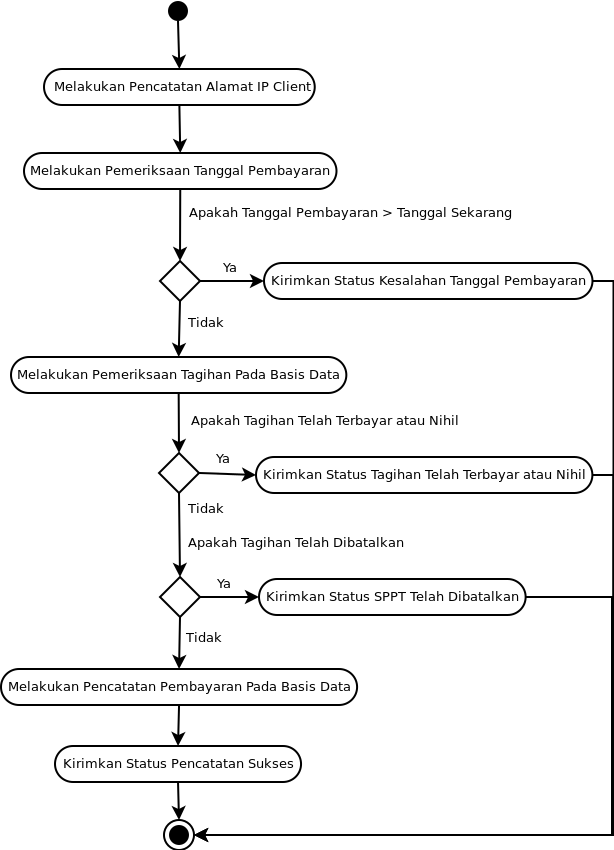
\includegraphics[width=0.8\textwidth]{./resources/uml/uml-act-bayar}
  \caption{Diagram \textit{Activity} Untuk Pencatatan Pembayaran}
  \label{fig:act-bayar}
\end{figure}

Aktivitas pencatatan pembayaran diawali pada saat \textit{client} melakukan \textit{request} pembayaran SPPT PBB-P2, \textit{server web services} akan melakukan pencatatan alamat IP darimana \textit{request} tersebut berasal.

Kemudian \textit{server} akan melakukan pemeriksaan terhadap tanggal pembayaran, apabila tanggal pembayaran melebihi tanggal saat dilakukannya proses pencatatan pembayaran, maka \textit{server} akan mengirimkan status kesalahan tanggal pembayaran ke \textit{client}, dan aktivitas selesai, namun bila tanggal pembayaran kurang dari atau sebelum hari dilakukannya proses pencatatan, maka aktivitas berlanjut ke proses berikutnya.

Pada tahap ini \textit{server} melakukan pemeriksaan tagihan pada basis data, apakah kondisi objek pajak (yang teridentifikasi dari nomor objek pajak) sudah terbayar atau belum, atau tagihannya nihil (tidak ada pajak yang terhutang), bila ya, maka \textit{server} akan mengirimkan status ke \textit{client} bahwa objek yang diminta telah terbayar atau merupakan objek yang piutangnya nihil. bila tidak, maka proses berlanjut.

Proses akhir dari aktivitas ini adalah melakukan pencatatan pembayaran pada basis data, kemudian mengirimkan status bahwa pencatatan tersebut telah selesai. Sampai sini aktivitas telah sampai pada ujung prosesnya.

\subsection{Diagram \textit{Activity} Untuk \textit{Reversal}}

Diagram \textit{activity} untuk melakukan proses \textit{reversal} adalah sebagaimana ditunjukkan pada gambar \ref{fig:act-reversal} :

\begin{figure}[H]
  \centering
  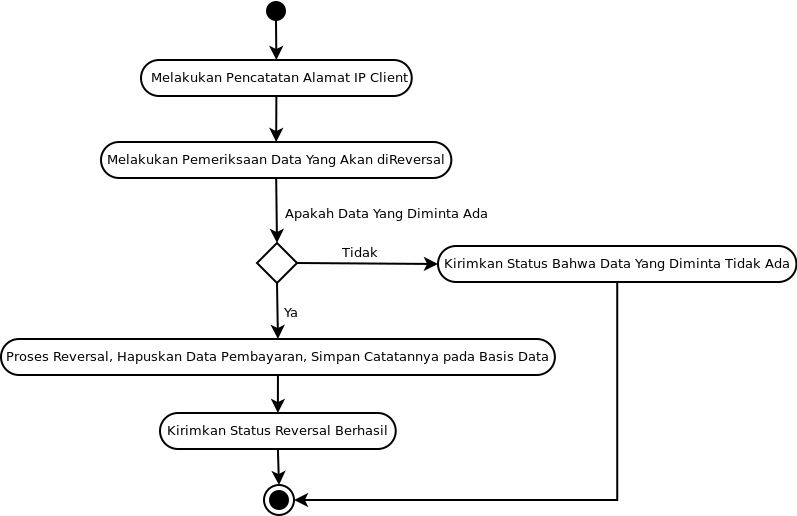
\includegraphics[width=0.8\textwidth]{./resources/uml/uml-act-reversal}
  \caption{Diagram \textit{Activity} Untuk Proses \textit{Reversal}}
  \label{fig:act-reversal}
\end{figure}

Seperti kedua aktivitas sebelumnya, hal yang pertama dilakukan adalah melakukan pencatatan alamat IP dari \textit{client}.

Kemudian melakukan pemeriksan data yang akan direversal, terutama terhadap Nomor Transaksi Pajak Daerah (NTPD) sebagai identitas sebuah transaksi. Apabila data NTPD ini salah, maka \textit{server} akan mengirimkan status kegagalan \textit{reversal} karena data yang diminta tidak ada. Bila data ada, maka melanjutkan ke proses berikutnya.

Langkah berikutnya adalah melakukan pencatatan \textit{request reversal} dan mengirimkan status ke \textit{client} bahwa \textit{reversal} yang diminta telah berhasil dilakukan.

Sampai sini aktivitas \textit{reversal} selesai.

Dari diagram \textit{use-case} dan diagram \textit{activity} telah didapat gambaran umum dari sistem aplikasi yang akan dibangun. Diagram-diagram berikutnya akan lebih detail membahas teknis bagaimana sistem bekerja.

\section{Diagram \textit{Class}}

Pada diagram \textit{class} ini, akan membahas detail dari tiap kelas pembentuk sistem aplikasi \textit{web services} secara keseluruhan. Karena akan menggunakan \textit{framework} Spring yang tentunya memiliki spesifikasi tersendiri, maka untuk memperjelas gambar diagram \textit{class} akan dibagi menjadi beberapa bagian, yaitu :

\begin{enumerate}
  \item Bagian Konfigurasi
  
  Bagian ini adalah kelas-kelas pembentuk konfigurasi \textit{framework} Spring sehingga aplikasi dapat dengan mudah dibangun tanpa perlu memikirkan detail teknis bagaimana Rest harus bekerja. Diagram \textit{class} dari bagian konfigurasi ini seperti ditunjukkan pada gambar \ref{fig:uml-class-konfig} :
  
  \begin{figure}[H]
    \centering
    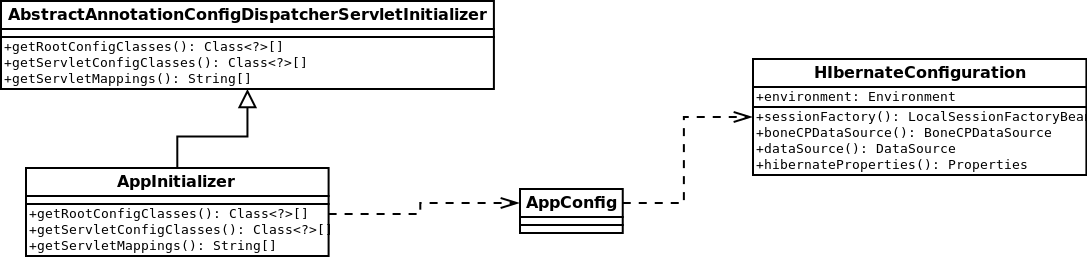
\includegraphics[width=1\textwidth]{./resources/uml/uml-class-konfig}
    \caption{Diagram \textit{Class} Bagian Konfigurasi \textit{Framework} Spring}
    \label{fig:uml-class-konfig}
  \end{figure}
  
  Kelas-kelas inilah yang nantinya mengatur \textit{services} dan konfigurasi koneksi dengan basis data. Awalnya \textit{servlet container} akan memanggil kelas AppInitializer hasil turunan dari kelas atau \textit{interface} AbstractAnnotationConfigDispatcherServletInitializer. Kelas AppInitializer ini membutuhkan kelas AppConfig untuk melakukan Konfigurasi khusus terkait struktur \textit{framework} Spring yang digunakan. Kelas AppConfig ini pun melakukan pemanggilan kelas HibernateConfiguration untuk melakukan konfigurasi komunikasi dengan \textit{server} basis data.
 
  \item Bagian \textit{Inquiry}
  
  Kelas-kelas pada bagian \textit{inquiry} ini, beberapa akan muncul pada bagian transaksi pembayaran ataupun \textit{reversal} karena kelas-kelas tersebut memiliki fungsi yang sama dalam siklus melayani \textit{request} dari \textit{client}. Kelas-kelas pada bagian \textit{inquiry} ini akan terlihat seperti pada gambar \ref{fig:uml-class-inquiry}
  
  \begin{figure}[H]
    \centering
    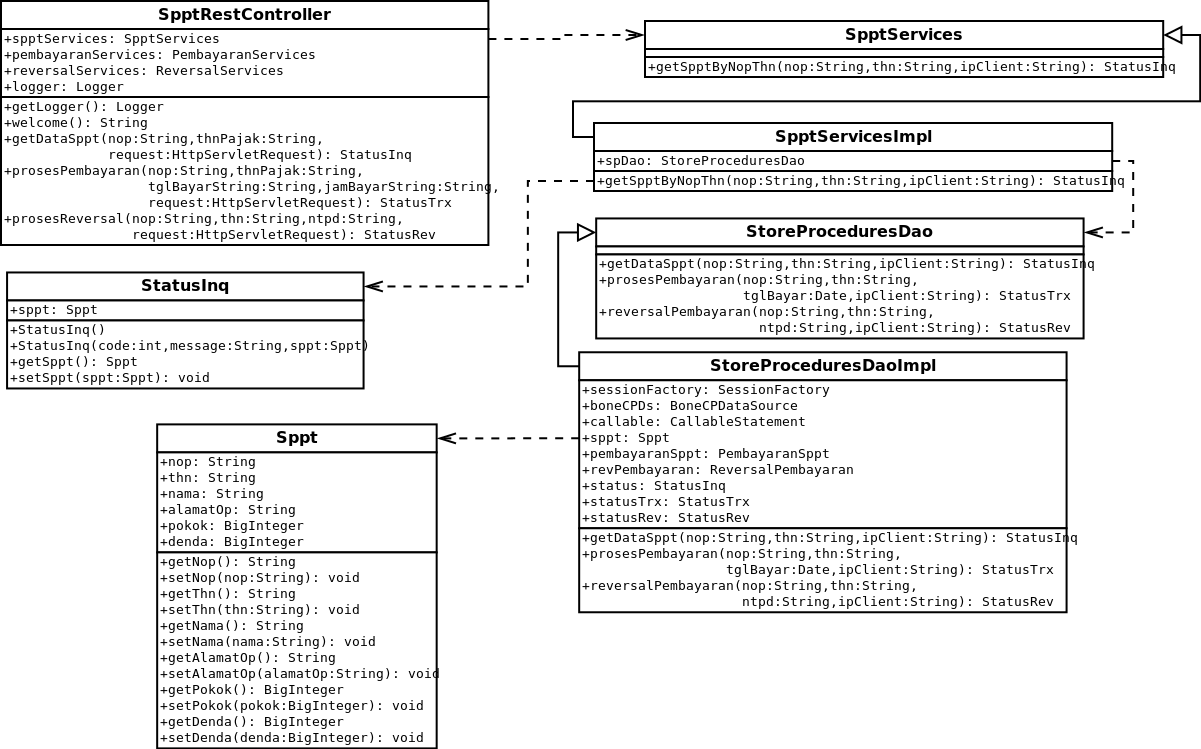
\includegraphics[width=1\textwidth]{./resources/uml/uml-class-inquiry}
    \caption{Diagram \textit{Class} Bagian \textit{Inquiry}}
    \label{fig:uml-class-inquiry}
  \end{figure}
  
  Kelas yang akan menjadi titik awal datangnya sebuah \textit{request} dari \textit{client} adalah kelas SpptRestController, kelas ini yang nantinya akan memilih apakah \textit{request client} adalah \textit{inquiry}, transaksi pembayaran, atau permohonan \textit{reversal}. Kelas SpptRestController ini pula yang nantinya mengirimkan pada \textit{service} yang berkaitan.
  
  Berkaitan dengan bagian \textit{inquiry}, maka begitu ada \textit{request inquiry} dikirimkan oleh \textit{client} dan diterima \textit{server} maka kemudian dipanggil \textit{interface} SpptServices, yang pada struktur kali ini diimplementasikan oleh kelas SpptServicesImpl.
  
  Karena \textit{framework} yang digunakan adalah Spring, maka diperlukan beberapa bagian berdasarkan fungsi utamanya. Fungsi dari masing-masing kelas yang berada pada \textit{framework} Spring yaitu :
  
  \begin{itemize}
    \item \textit{Domain Object}. Kelas-kelas yang memiliki fungsi ini mewakili struktur data persis seperti pada basis data. Penggunaan kelas-kelas pada \textit{domain object} diperlukan karena :
    
    \begin{enumerate}[1)]
      \item Kode program jadi lebih mudah dimengerti dan dipelihara.
      \item Karena Java merupakan bahasa yang \textit{strongly-typed} dan harus di-\textit{compile} terlebih dahulu, akan memudahkan pemeriksaan \textit{bug} pada saat \textit{compile} dibandingkan saat \textit{runtime} atau berjalannya aplikasi.
      \item Memisahkan lapisan data dan antarmuka / \textit{interface}. Apabila ada perubahan skema pada basis data tetapi fitur pada tampilan antarmuka tidak berubah, maka cukup dilakukan perubahan pada lapisan data / \textit{domain object}-nya saja.
      \item Pustaka siap pakai untuk validasi. Di Java, ada pustaka yang berguna untuk melakukan validasi, yaitu JSR-303. Terhadap validasi data yang akan dimasukkan ke dalam basis data, kita tidak perlu melakukan pengecekan seperti contoh kode berikut :
      
      \begin{lstlisting}[language=java]
      if(mydata.getId() == null)
      \end{lstlisting}
      
      Melainkan cukup dengan kode berikut :
      
      \begin{lstlisting}[language=java]
      @NotNull private String Id;
      \end{lstlisting}
    \end{enumerate}
    
    \item \textit{Interface Business Services}
    
    Kelas-kelas pada fungsi ini hanya berupa definisi daftar fitur yang disediakan oleh aplikasi. Seluruh implementasi dikelas ini belum terisi, oleh karena itu dinamakan \textit{interface}. Beberapa alasan penggunaan \textit{interface} atau kelas-kelas abstrak atau tanpa implementasi ini adalah sebagai berikut :
    
    \begin{itemize}
      \item Pada saat membangun sebuah aplikasi \textit{client-server}, maka cukup dengan memberikan kelas-kelas pada \textit{domain object} dan \textit{interface} ini pada \textit{programmer} yang membangun sisi \textit{client}, tanpa perlu menyertakan implementasi dari \textit{interface} yang biasanya cukup besar, aplikasi dapat saling berkomunikasi.
      
      \item Pada saat ada peralihan atau perubahan implementasi perangkat lunak basis data, maka aplikasi disisi \textit{client} tidak perlu berubah.
      
      \item Fitur \textit{declarative transaction} yang dimiliki Spring akan lebih optimal bekerja bila dipisahkan antara \textit{interface} dengan implementasinya.
    \end{itemize}
    
    \item \textit{Implementasi Business Services}
    
    Ini adalah bagian dari implementasi \textit{interface business services}. Jika pada \textit{interface} berisi fitur abstrak, pada bagian ini sudah ada implementasi konkrit untuk masing-masing fitur yang telah didefinisikan pada \textit{interface}. Karena sistem aplikasi akan menggunakan Spring Data JPA, maka diperlukan kelas-kelas lain selain \textit{business services}, yaitu kelas-kelas implementasi \textit{Data Access Object} (DAO).
  \end{itemize}
  
  Implementasi dari kelas SpptServicesImpl akan mengembalikan kelas StatusInq sebagai respon terhadap \textit{request} yang telah sampai ke \textit{server}. Kelas SpptServicesImpl membutuhkan paket kelas DAO berupa \textit{interface} StoreProceduresDao untuk melakukan komunikasi dengan basis data. Implementasi dari \textit{interface} StoreProceduresDao ini adalah kelas StoreProceduresDaoImpl dimana implementasi didalamnya akan menggunakan kelas Sppt untuk menyimpan atau menampung nilai-nilai yang dihasilkan dari pemanggilan \textit{store procedure} pada basis data. Yang pada akhirnya akan dikembalikan kelas Sppt ini dalam bentuk yang terbungkus dalam kelas StatusInq.
  
  \item Bagian Transaksi Pembayaran
  
  
  
  \item Bagian \textit{Reversal}
\end{enumerate}

\section{Diagram \textit{Sequence}}

\section{Diagram \textit{Statechart}}
